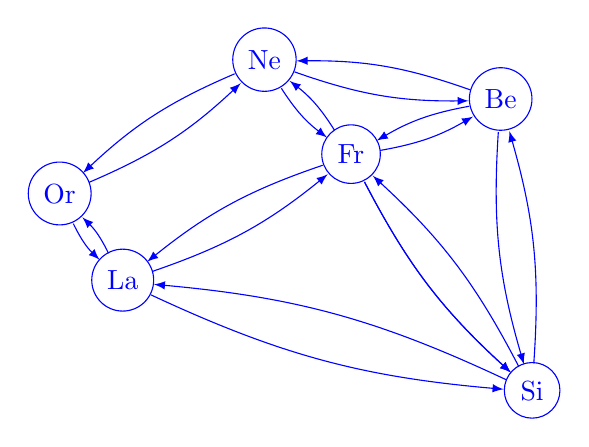
\begin{tikzpicture}[blue, scale=6]
  \node[draw, circle] (LA) at (6.6667, 46.5333) {La};
  \node[draw, circle] (BE) at (7.4667, 46.9167) {Be};
  \node[draw, circle] (NE) at (6.9667, 47){Ne};
  \node[draw, circle] (FR) at (7.15, 46.8) {Fr};
  \node[draw, circle] (OR) at (6.5333, 46.7167) {Or};
  \node[draw, circle] (SI) at (7.5333, 46.3) {Si};

  \draw[-latex] (LA) to[bend right=10] (OR) ;
  \draw[-latex] (LA) to[bend right=10] (FR) ;
  \draw[-latex] (LA) to[bend right=10] (SI) ;
  \draw[-latex] (BE) to[bend right=10] (NE) ;
  \draw[-latex] (BE) to[bend right=10] (FR) ;
  \draw[-latex] (BE) to[bend right=10] (SI) ;
  \draw[-latex] (NE) to[bend right=10] (OR) ;
  \draw[-latex] (NE) to[bend right=10] (FR) ;
  \draw[-latex] (NE) to[bend right=10] (BE) ;
  \draw[-latex] (FR) to[bend right=10] (LA) ;
  \draw[-latex] (FR) to[bend right=10] (NE) ;
  \draw[-latex] (FR) to[bend right=10] (BE) ;
  \draw[-latex] (FR) to[bend right=10] (SI) ;
  \draw[-latex] (FR) to[bend right=10] (SI) ;
  \draw[-latex] (OR) to[bend right=10] (NE) ;
  \draw[-latex] (OR) to[bend right=10] (LA) ;
  \draw[-latex] (SI) to[bend right=10] (LA) ;
  \draw[-latex] (SI) to[bend right=10] (FR) ;
  \draw[-latex] (SI) to[bend right=10] (BE) ;
\end{tikzpicture}
